\documentclass{article}
\usepackage[utf8]{inputenc}
\usepackage{titlesec}
\titleformat*{\subsection}{\normalsize\bfseries}
\usepackage[square,sort,comma,numbers]{natbib}
\usepackage[nottoc,numbib]{tocbibind}
\usepackage{relsize}
\usepackage{csquotes}
\usepackage{natbib}
\usepackage{graphicx}
\usepackage{verbatim}
\usepackage{float}
\usepackage{verbatim}
\usepackage{caption}
\usepackage{subcaption}
\usepackage{url}
\usepackage{listings}
\usepackage{xcolor}
\definecolor{listinggray}{gray}{0.9}
\definecolor{lbcolor}{rgb}{0.9,0.9,0.9}
\lstset{
		backgroundcolor=\color{lbcolor},
		tabsize=4,    
		language=[GNU]C++,
		basicstyle=\scriptsize,
		%upquote=true,
		aboveskip={1.5\baselineskip},
		columns=fixed,
        showstringspaces=false,
        extendedchars=false,
        breaklines=true,
        prebreak = \raisebox{0ex}[0ex][0ex]{\ensuremath{\hookleftarrow}},
        frame=single,
        numbers=left,
        showtabs=false,
        showspaces=false,
        showstringspaces=false,
        identifierstyle=\ttfamily,
        keywordstyle=\color[rgb]{0,0,1},
        commentstyle=\color[rgb]{0.026,0.112,0.095},
        stringstyle=\color[rgb]{0.627,0.126,0.941},
        numberstyle=\color[rgb]{0.205, 0.142, 0.73}
}
\lstset{
    backgroundcolor=\color{lbcolor},
    tabsize=4,
  language=C++,
  captionpos=b,
  tabsize=3,
  frame=lines,
  numbers=left,
  numberstyle=\tiny,
  numbersep=5pt,
  breaklines=true,
  showstringspaces=false,
  basicstyle=\footnotesize,
  keywordstyle=\color[rgb]{0,0,1},
  commentstyle=\color{Darkgreen},
  stringstyle=\color{red}
  }


\title{3 fundamental problems in algorithm engineering}
\author{Benjamin Blankholm \\
		E-mail: benner@cs.au.dk \\
		Study nr. 201206087}

\date{\today}

\begin{document}

\maketitle
\newpage

\section{Introduction}
In this report 3 projects will be described, and analyzed. The projects are looking into optimizing algorithms, for search, matrix multiplication, and sorting. These three fields of algorithm engineering, are fundamental problems with wide spread use.
This report looks into the three projects with a goal of improving the simpler and more theoretical algorithms, with respect to running time on real computers. This involves reasoning about the hardware architecture, and taking into account the evolution of modern systems. 

\section{Binary Search}
In this project we have tried to optimize a regular binary search algorithm, by changing the split point and by changing the memory layout of the data searched. The project seeks to find a suitable data structure to support the \textit{pred} operation. 
\begin{center}
$Pred(x) = return \max \{ y \in S | y \leq x \}$	
\end{center}

\subsection{Modern hardware}
\label{sec:modern_hardware}
It is a well known fact, that using asymmetrical splits in algorithms in some cases result in better performance. %TODO REF
This is usually caused by the hardware architecture of modern computers. In modern CPUs long computation pipelines is used to compute multiple instructions in sequence. This means, that often it will be necessary for the CPU to try and predict which branch of instructions the execution of the program will take, and stick it in the computation pipeline. If this prediction turns out to be wrong, the computations of the instructions in the wrong branch is effectively wasted work. This is known as a branch misprediction. It turns out, that in some cases it can be beneficial to make these branching statements easier to predict. This can be done by making the branching statement take the one path of execution more often than the other. Exactly how much bias is needed toward one of the branches, is not clear. 

An other known factor to influence running time, is cache and Translation Lookaside Buffer (TLB) misses. Because it is possible to make smaller memory sizes work faster, the memory architecture of modern computers is a hierarchy. This hierarchy contains in most desktop computers three layers of cache, Random Access Memory (RAM), and disk storage. Here the three layers of cache is known as L1, L2 and L3. Multicore CPUs are often structured such that each individual core has its own dedicated L1, and L2 caches, whereas the L3 cache is shared between the cores. Here the L1, is the smallest level of cache, but the fastest, whereas L3 is largest and slowest of the three L2 is somewhere in between. RAM is however a lot larger, than the small caches, so if the program running is using data that is too large to fit in the cache, some replacement of values in the caches must be performed during the execution of the program. 
When a program needs some resource stored in memory, it will look for it in the cache. If it is not present in the cache a cache miss occurs. This means that the resource must be found in a higher level of cache, og in main memory. If the resource is only located in main memory, a lookup in the TLB will be performed to get the address in physical memory.\footnote{In computer architecture one operates with mainly two kinds of memory, virtual and physical memory. Virtual memory, is used to hide the implications of having physical addresses. This means, that it seems like to the individual application, that it has the entire address space available. It also means, that a virtual address (the addresses the applications use) must be mapped to a physical address such that it can actually be stored.} If the address is pressent in the TLB a TLB hit occurs, and the physical address can be looked up almost instantly. If however the address is not pressent int the TLB a TLB miss occurs, and this causes a page walk, which requires several memory lookups.
The TLB and the caches are ordered in such a way, that the resources are stored in sequential blocks. In the cache the data is loaded in cache lines, and the TLB is working with pages. This means that it is beneficial to access the resources used in a sequential manner whenever possible, because it will most often cause less pagewalks, and cache misses.

\subsection{Improvements to binary search}
\label{sec:improvements}
In order to meet the complications that arises from modern hardware architecture discussed in section \ref{sec:modern_hardware}, some specific design choices has been made. One possible improve ment is to try and limit the amount of branch mispredictions to gain better performance from less waisted computing time. This is done by trying to skew the split of the search space, in order to make it more plausible for the binary search algorithm to find the result in the one side rather than the other. If the algorithm is searching for a value on a randomly uniform data structure and the algorithm is splitting the data structure in half, one would expect that there is a 50/50 chance of finding the value in either of the two partitions. This would result in a large amount of branch mispredictions, and thus it might be better to make an other partitioning. On figure \ref{fig:array_split} two different splits of an array is shown. In the tests of the algorithm a \textit{skew} is used, to determine the split-point for the algorithm. This \textit{skew} is a number between 0 and 1, where 0.5 would result in a 50/50 split, and 1 or 0 would result in the entire data structure being on the one side of the split, such that the binary search effectively would become a linear search.

\begin{figure}[H]
  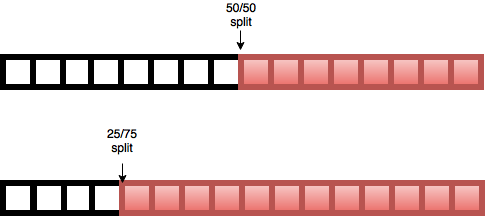
\includegraphics[width=\textwidth]{figures/Array_eq_split}
  \caption{An array split 50/50, compared to an array split 25/75}
  \label{fig:array_split}
\end{figure}

Besides skewing the partitioning of the data structure, the data is stored as a Binary Search Tree (BST). The simplest way of storing the data for a binary search would be using a sorted array. However this approach would result in a large amount of cache misses and pagewalks, because the read from memory would be nothing like sequential. The recursive algorithm would take logarithmic steps in memory. 

As opposed to the sorted array, three different memory layouts of a BST has been studied. These being a Breadth First Search (BFS) manor, a Depth First Search left (DFSl) manor, and a Depth First Search right (DFSr) manor. Figure \ref{fig:BST_layouts} shows how the different layouts of BSTs are structured in memory. These layouts were chosen because of their simplicity, and their properties with respect to memory addresses when skewing the data structure. The hope for the DFSl layout is that it will perform well when the data structure is skewed to the left. The combination of high probability of visiting the left child of a node, and the fact that the left child is the next memory address, could potentially mean that there will be both less branch mispredictions and less cache misses and pagewalks.

\begin{figure}[H]
  \centering
  \begin{subfigure}[b]{0.51\textwidth}
  	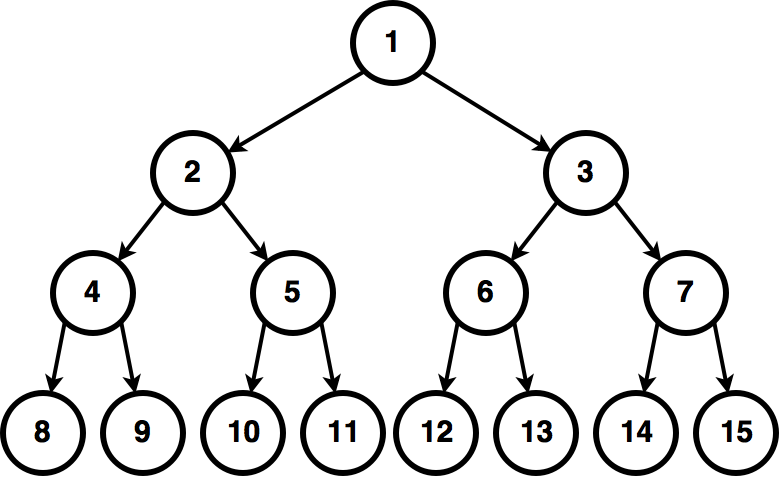
\includegraphics[width=\textwidth]{figures/BFS_layout}
  	\caption{BFS layout}
  \end{subfigure}
  \begin{subfigure}[b]{0.49\textwidth}
    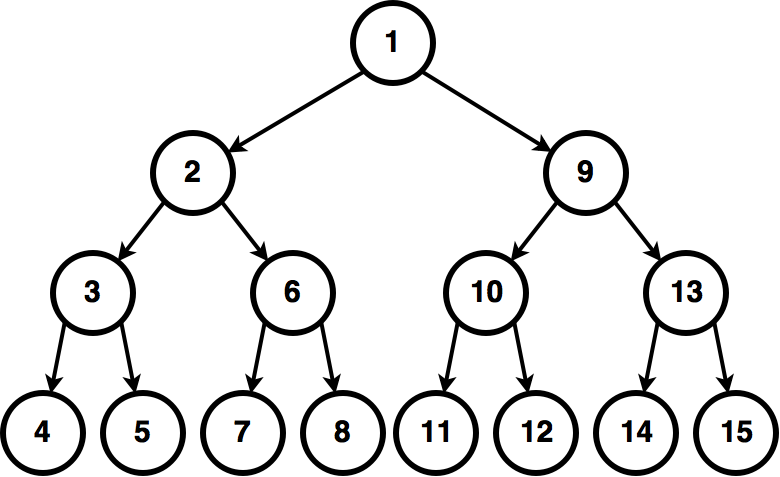
\includegraphics[width=\textwidth]{figures/DFSl_layout}	
    \caption{DFSl layout}
  \end{subfigure}
    \begin{subfigure}[b]{0.49\textwidth}
    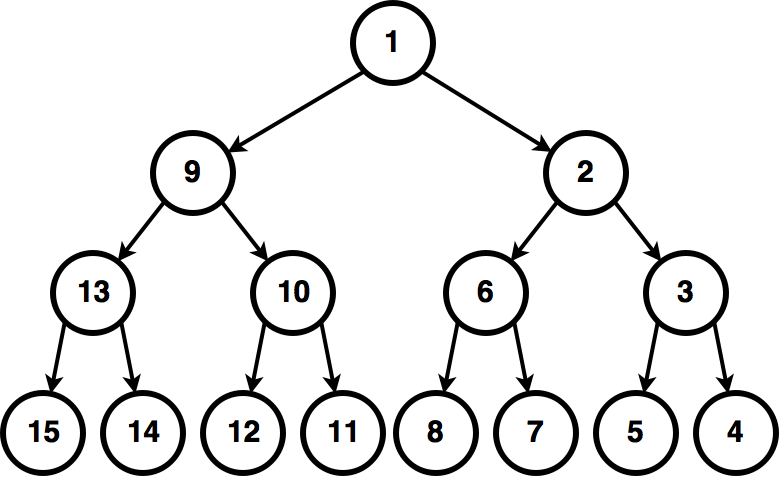
\includegraphics[width=\textwidth]{figures/DFSr_layout}	
    \caption{DFSr layout}
  \end{subfigure}
  \caption{The BSTs with numbers representing the relative positioning of the nodes in memory, for each of the three types of layout.}
  \label{fig:BST_layouts}
\end{figure}

\subsection{Implementation}
Because the tests performed are carried out on BSTs the binary search implementation looks as in figure \ref{code:binary_search_bst}. The implementation takes the Node (which is shown in figure \ref{code:node}) from the first index in the array. This is defined to be the root of the tree in all of the three memory layouts. And by the definition of the BST this would be the first node to be checked by the binary search algorithm. From the root the algorithm simply follows the pointers according toward the better matching value, until it finds the best match for the search.

\begin{figure}[H]
  \centering
  \begin{lstlisting}
int binary_search_on_bst(int s, Node array[]) {
  Node current_node = array[0];

  while(current_node.val != s){
    if(current_node.val > s && current_node.left != NULL) {
      current_node = *current_node.left;
    } else if(current_node.val < s 
    		  && current_node.right != NULL 
  		      && current_node.right->val < s) {
      current_node = *current_node.right;
    } else {
      break;
    }
  }

  return current_node.val;
};
  \end{lstlisting}
  \caption{Implementation of binary search on a BST in C++}
  \label{code:binary_search_bst}
\end{figure}

\begin{figure}[H]
	\centering
	\begin{lstlisting}
struct Node{
  int val;
  Node *left;
  Node *right;

  Node(){}
  
  Node(int v, Node *l, Node *r){
    this->val = v;
    this->left = l;
    this->right = r;
  }
};
	\end{lstlisting}
	\caption{The C++ representation of a BST node}
	\label{code:node}
\end{figure}

To construct the skewed BST the algorithm in figure \ref{code:build_bst} is used. This algorithm constructs the nodes and pointers, in such a way that the resulting BST becomes skewed with the provided fraction.

\begin{figure}[H]
	\centering
	\begin{lstlisting}
Node* build_BST(int in[], int L, int H, double skew){
  if(L>=H) return NULL;

  int i = L + floor((H-L)/(1/skew));

  if(i == L){
    return new Node(in[i],
		    NULL,
		    build_BST(in, L+1, H, skew));
  }
  if(i == H){
    return new Node(in[i],
		    build_BST(in, L, H-1, skew),
		    NULL);
  }
  
  return new Node(in[i],
		  build_BST(in, L, i, skew),
		  build_BST(in, i+1, H, skew));
};
	\end{lstlisting}
	\caption{An algorithm for building a skewed BST from a sorted array}
	\label{code:build_bst}
\end{figure}

When the BST is constructed it can be placed in memory according to the layouts described in section \ref{sec:improvements}. This is done by three different functions. (one for each layout) The algorithms are recursively laying out the nodes in memory, ensuring the correct placement in memory. This is done by constructing an array of nodes of the same length as the size of the BST. The nodes from the original BST are then copied into the new array in such a way, that they will fulfill the constraints of the desired layout.The algorithm for laying out the BST in a DFSl manor can be found in figure \ref{code:dfsl_layout}.

\begin{figure}[H]
	\centering
	\begin{lstlisting}
int tree_to_dfsl(int index, Node* current_node){
  dfsl_array[index].val = current_node->val;

  int next_index = index+1;
  if(current_node->left != NULL){
    dfsl_array[index].left = &dfsl_array[next_index];
    next_index = tree_to_dfsl(next_index, current_node->left);
  }
  
  if (current_node->right != NULL) {
    dfsl_array[index].right = &dfsl_array[next_index];
    next_index = tree_to_dfsl(next_index, current_node->right);
  }

  return next_index;
};
	\end{lstlisting}
	\caption{The algorithm for laying out a BST in DFSl in memory}
	\label{code:dfsl_layout}
\end{figure}

\subsubsection{Implementation challenges}
During the implementation of the algorithms for skewing and laying out the trees several challenges were found. The major problem was that the most obvious way to lay out a BST in a BFS manor, would not work for very skewed instances, because there would be large holes in the array, and the program would quickly run out of memory addresses. \footnote{In the straight forward BFS layout of a BST, the left child of a node would be found at the address of the node itself multiplied by two, and the right child would be found on the same address as the left plus one.} To solve this problem, and give the BFS layout a fighting chance in the tests, an other way of laying out the BST was designed. For this a new node type was used, which besides the two pointers and the value could also hold an index, which would represent the array index of the node. With this type of node it is possible to first build a BST from the new heavy nodes, and then run through the nodes and assign indexes to them. When this is done the tree of heavy nodes is the copied into an array of regular nodes, such that the extra index value in the struct would not cause any inconsistencies in the tests. The algorithm for assigning the indexes to the nodes can be found in figure \ref{code:bfs_index}. This algorithm ensures that there will be no holes in the array, so all of the layouts would take up an equal amount of space in memory.

\begin{figure}[H]
	\centering
	\begin{lstlisting}
void bfs_index_heavy_tree(HeavyNode * root){
  int index = 0;

  queue<HeavyNode*> queue;
  queue.push(root);
  while(!queue.empty()){
    HeavyNode * current_node = queue.front();
    queue.pop();

    current_node->index = index;

    if(current_node->left != NULL){
      queue.push(current_node->left);
    }

    if(current_node->right != NULL){
      queue.push(current_node->right);
    }
    index++;
  }
  return;
};
	\end{lstlisting}	
	\caption{The algorithm for assigning indexes to nodes in a BFS manor}
	\label{code:bfs_index}
\end{figure}


\subsection{Performed tests}
\textit{Skews} between 0.05 and 0.95 (0.05 size steps) has been tested using the different memory layouts. During the tests five different hardware counters has been monitored. These being the number of branch mispredictions, the number of times the hardware prefetchers causes a cache miss in L2 cache, the number of request for ownership (RFO) that misses L2 cache, the number of requests missing L3, and the number of misses in TLB that causes a pagewalk.
Besides these hardware counters, the running time of the algorithm using the different skews has been measured as well.
The algorithm has been tested on arrays of size 1,000,000 and 10,000,000. The hope is to show a larger difference in TLB misses for high and low \textit{skews} using the larger dataset. During each test the \textit{pred} query is run as many times as there is indices in the data structure. This means, that if the data structure contains 10,000,000 nodes, 10,000,000 lookups for random numbers will be performed. 

From the tests one could expect to see that the curves for the running time would increase when gets closer to 0.5, and again when it is nearing the outer edges (0 and 1) where the algorithm will start to perform more like a linear search. Where usually binary search has a time complexity of $O(\log n)$ linear search has a time complexity of $O(n)$, which is the reason for the expected increase in running time toward the edges. On the other hand the findings from %TODO REF
indicates that the running time could increase where a lot of branch mispredictions are likely to occur. With this put together one could expect to see a dip in running time as the skew moves away from 0.5 to either side. An other factor which should be taken into account is that the depth first layouts combined with a skew could result in a further increase in performance, because less cache faults and TLB misses are likely to occur. The reason is, that with a high skew (in the range $]0.5;1]$) the majority of the nodes will be in the left subtree, and with a DFSl layout, they will furthermore be placed on sequential addresses in memory. Because of these factors a skew in the range $]0.5;1]$ and a DFSl layout is expected to result in fewer branch mispredictions, and fewer cache faults which in in turn could result in better performance.

\subsection{Results}
As expected the number of branch mispredictions, when running the tests for different \textit{skews} decreases with a more skewed data structure. Figure \ref{fig:branch_misses} shows the trend of branch mispredictions decreasing as the skew moves away from 0.5. Very similar results were found for both DFSl and DFSr, which is as expected since the branching would not change because of changes in memory addresses for the nodes.

\begin{figure}[H]
	\centering
	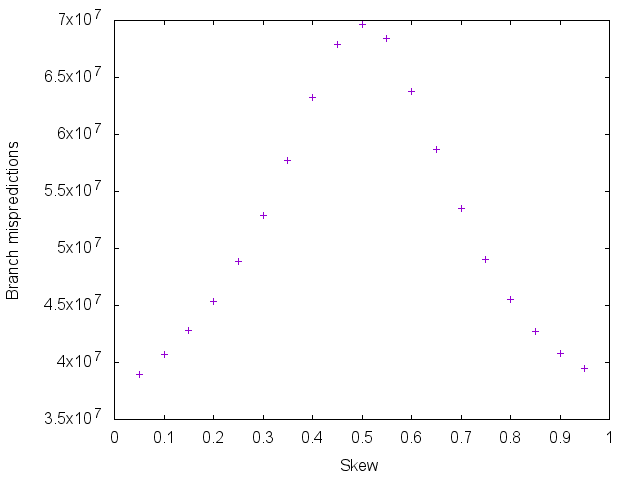
\includegraphics[width=0.7\textwidth]{figures/BFS_branch_misses}
	\caption{The number of branch mispredictions using BFS layout with different \textit{skew}}
	\label{fig:branch_misses}
\end{figure}

From figure \ref{fig:TLB_misses_BFS} it can be seen that the number of TLB misses increases when the data structure is less balanced. A notable increase starts when the skew passes 0.2 and 0.8. Because a pagewalk is an expensive operation compared to clock cycles or cache requests, it may therefor be expected that the running time would also increase a fair amount when the skew passes these points. Likewise a similar trend can be seen for L2 cache misses in figure \ref{fig:L2_RFO_misses_BFS}.

\begin{figure}[H]
	\centering
	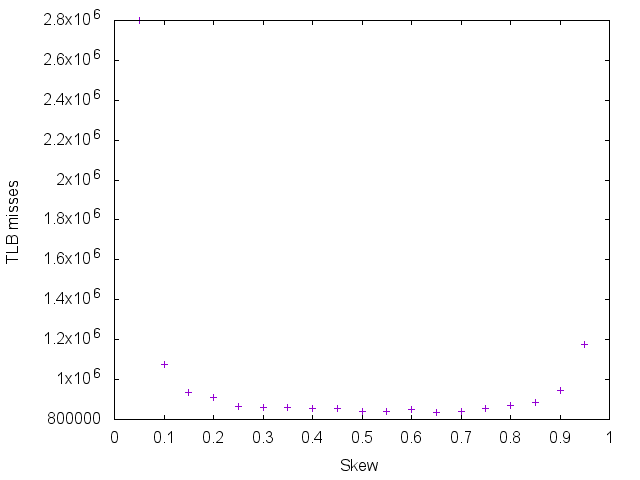
\includegraphics[width=0.7\textwidth]{figures/BFS_TLB_misses}
	\caption{The number of TLB misses that causes a pagewalk when using BFS layout}
	\label{fig:TLB_misses_BFS}
\end{figure}

\begin{figure}[H]
	\centering
	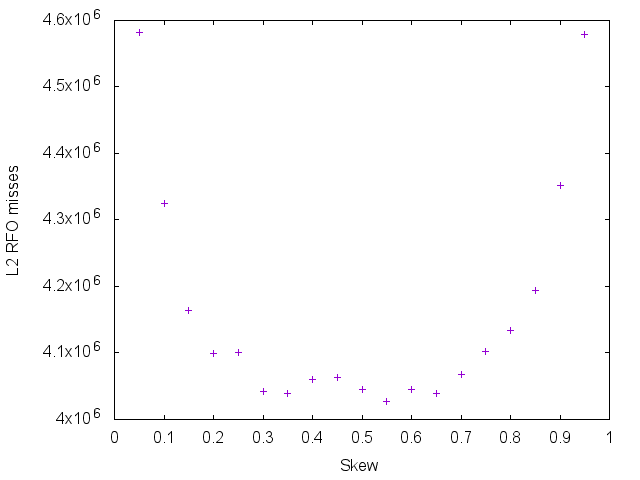
\includegraphics[width=0.7\textwidth]{figures/BFS_L2_RFO_misses}
	\caption{The number of cache faults caused by RFO requests, when using BFS layout}
	\label{fig:L2_RFO_misses_BFS}
\end{figure}

A quite different pattern can be seen in the counts for the L3 cache misses in figure \ref{fig:L3_misses_BFS}. Here the number of cache misses starts to decrease when the skew goes toward the two extremes (When the skew goes below 0.25 or when it exceeds 0.75). The reason for this could be that the data structure gets skewed enough for the sought after nodes to be placed close enough to each other in memory for the addresses to fit in the L3 cache. This would happen in cases where the tree is so unbalanced that several child nodes in sequence would have only one child. This would mean that the size of the layers in the tree would not increase all the way to the bottom layer, but rather at some point the size of the layers would start to decrease when moving down through the tree. This could result in an entire subtree being able to fit in a cache line of the L3 cache, and thus fewer misses would occur when moving through this sub tree.

\begin{figure}[H]
	\centering
	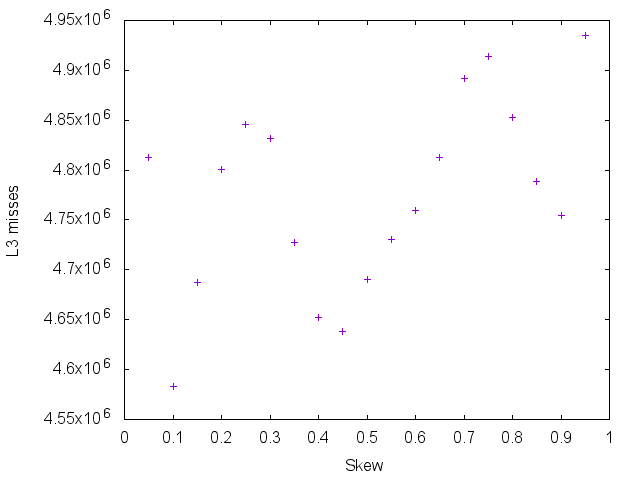
\includegraphics[width=0.7\textwidth]{figures/BFS_L3_misses}
	\caption{The number of L3 cache misses, when using BFS layout}
	\label{fig:L3_misses_BFS}
\end{figure}

In figure \ref{fig:combined_misses} all the tests for all three memory layouts are put together. It is clear that the depth first memory layouts performs better in terms of cache misses and TLB misses, as expected. In all of the plots the BFS layout is causing around 20\% more misses than the DFSl and DFSr layouts. It may also be seen that the plots for the L3 cache misses for DFSl and DFSr is more uniform than BFS (figure \ref{fig:L3_misses_BFS} discussed in the previous paragraph). This can be explained from the fact that if the data structure (when using DFS) is less balanced, there will be a larger chance of the node placed sequentially in memory being the next visited by the algorithm. And because memory is used in blocks, either as cache lines, or as pages, accessing the memory sequentially will in all likelihood mean that the next resource used is already loaded.

However when this all comes together, it is not immediately evident, that the depth first layouts actually perform better than BFS when looking at the running time. The curves found in figure \ref{fig:combined_running_time} seem to agree largely with the curvatures of the plots of the different cache misses and TLB misses. But the increase increase in cache misses from the depth first layouts to the BFS layout, does not seem to be enough of a change to make a notable difference on the running time. It could be however that the branch mispredictions is more of a dominating factor, which might explain why the running times around a \textit{skew} of 0.5 is a bit larger than the running times for less balanced trees.

\begin{figure}[H]
	\centering
	\begin{subfigure}[b]{0.49\textwidth}
		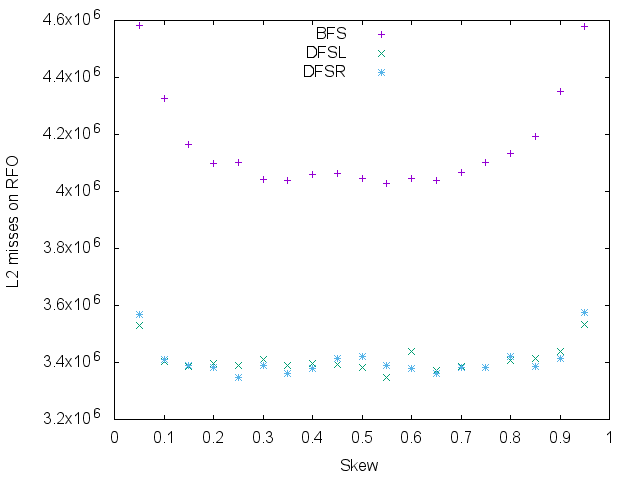
\includegraphics[width=\textwidth]{figures/combined_L2}	
	\end{subfigure}
	\begin{subfigure}[b]{0.49\textwidth}
		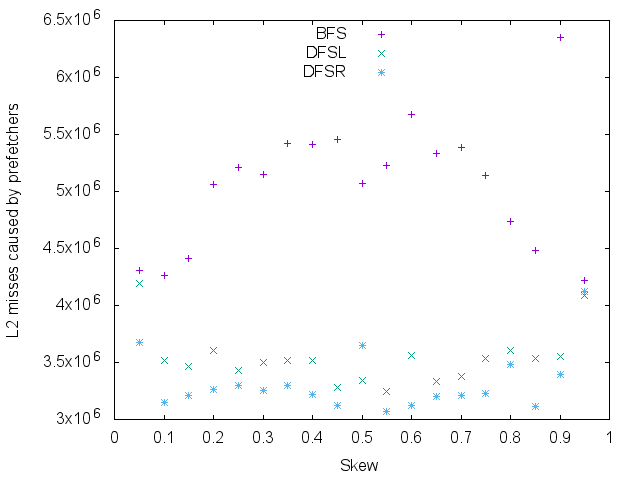
\includegraphics[width=\textwidth]{figures/combined_L2_PF}	
	\end{subfigure}
	\begin{subfigure}[b]{0.49\textwidth}
		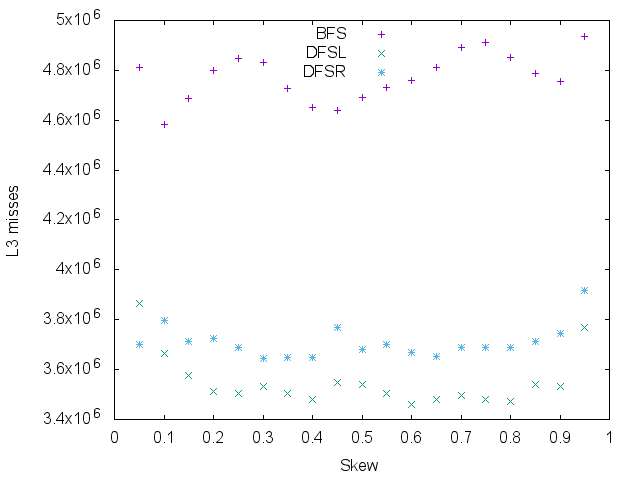
\includegraphics[width=\textwidth]{figures/combined_L3}	
	\end{subfigure}
	\begin{subfigure}[b]{0.49\textwidth}
		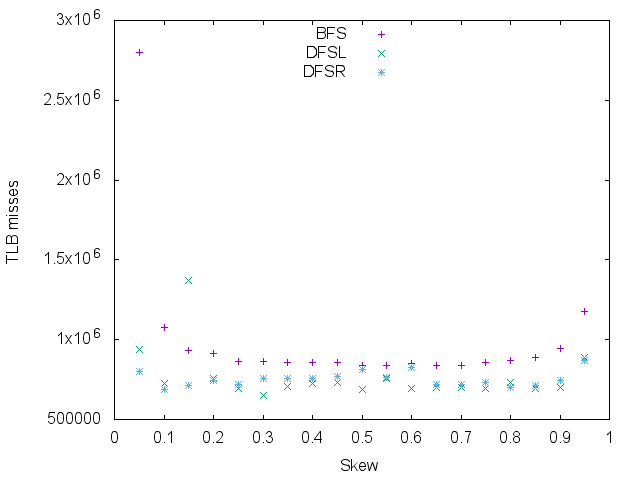
\includegraphics[width=\textwidth]{figures/combined_TLB}	
	\end{subfigure}
	\caption{Combined plots of cache misses and TLB misses for the three different memory layouts}
	\label{fig:combined_misses}
\end{figure}

\begin{figure}[H]
	\centering
	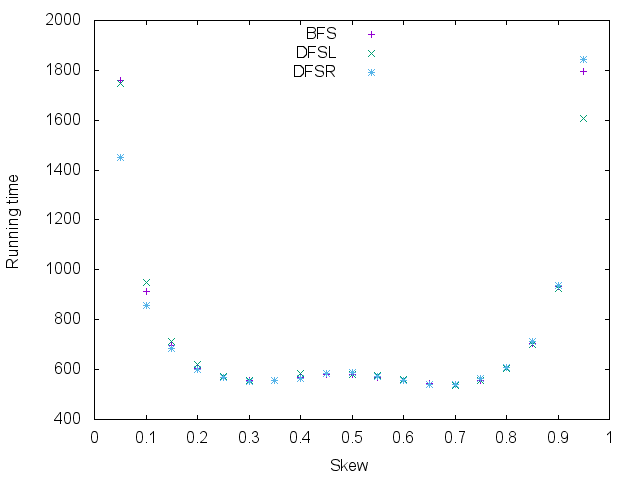
\includegraphics[width=0.7\textwidth]{figures/combined_running_time}
	\caption{Combined plots of running times for the three different memory layouts}
	\label{fig:combined_running_time}
\end{figure}

From figure \ref{fig:combined_running_time} it looks like a \textit{skew} of 0.7 is preferable so a test of different data sizes has been made to compare the running times using this \textit{skew}. The result of this test can be found in figure \ref{fig:combined_running_time_07}. In this figure it is again evident, that the different layouts does not seem to make much of a difference to the running time of the algorithm. Oun could expect that the DFSl layout would be superior because the BST would be unbalanced to the left when using a \textit{skew} of 0.7. However et seems that if anything DFSr is actually performing a tiny bit better.

\begin{figure}[H]
	\centering
	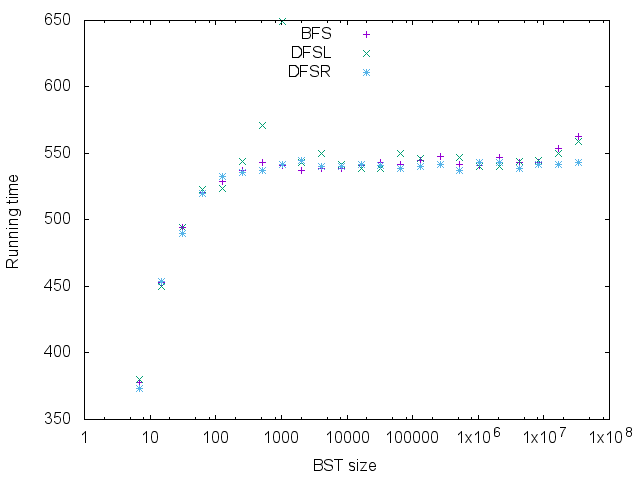
\includegraphics[width=0.7\textwidth]{figures/combined_running_time_07}
	\caption{Running time for increasing sizes of the BST, using the three different memory layouts.}
	\label{fig:combined_running_time_07}
\end{figure}

\subsection{Conclusion}
In this project it has been shown that using BSTs, the memory layout of the tree has a rather large impact on the amount of cache misses as well as TLB misses. BFS, DFSl and DFSr has been studied, and the depth first layouts has shown to cause a notable amount less cache misses and TLB misses. Along with branch mispredictions decreasing, with unbalancing the BST, it was expected that the DFS layouts would perform better than the BFS layout, but sadly the tests performed failed to show a notable difference in running time.

It may be that larger data sizes would need to be used in order to see a performance gain. If larger data sizes had been used more TLB misses would be expectable, and this may cause a notable difference to the running time. Unfortunately we have not been able to test this hypothesis because of lack of time. 

\subsection{How To run the code}
The main code for this project can be found in \texttt{binary\_search\_BST.cpp}. The main function of the program takes as arguments the desired size of the BST to be generated and tested on, as well as the desired \textit{skew}. If the desired size of the BST is chosen to be $<=0$ the program will do a test run, comparing the running time on the three different memory layouts on increasing sizes of BSTs.

\section{Matrix Multiplication}

\subsection{Performed tests}
\subsection{How To run the code}

\section{Improving Javas Quick Sort}
\subsection{Performed tests}
\subsection{How To run the code}



\end{document}
